\begin{figure}[H]
	\centering
	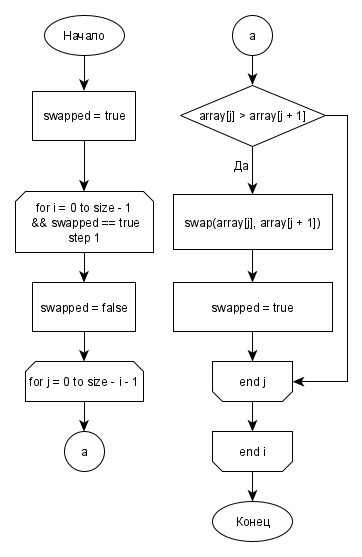
\includegraphics[width=0.7\linewidth]{../Рисунки/bubble}
	\caption{Схема сортировки пузырьком}
	\label{fig:bubble}
\end{figure}

\begin{figure}[H]
	\centering
	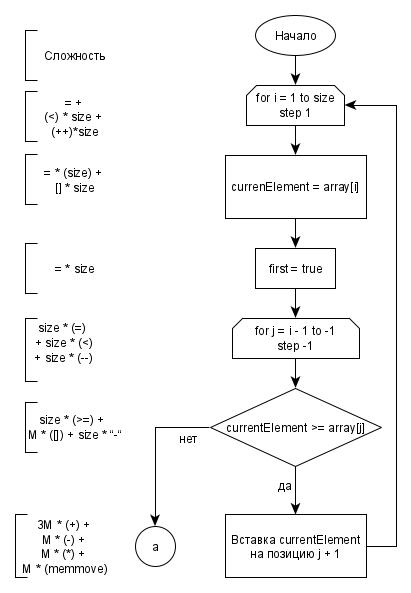
\includegraphics[width=0.7\linewidth]{../Рисунки/insertion1}
	\caption{Cортировка вставками схема 1}
	\label{fig:insertion}
\end{figure}

\begin{figure}[H]
	\centering
	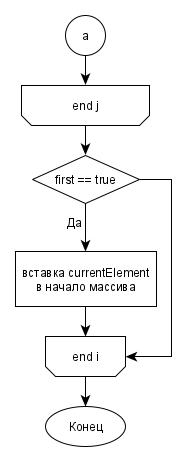
\includegraphics[width=0.7\linewidth]{../Рисунки/insertion2}
	\caption{Сортировка вставками схема 2}
	\label{fig:insertion2}
\end{figure}


\begin{figure}[H]
	\centering
	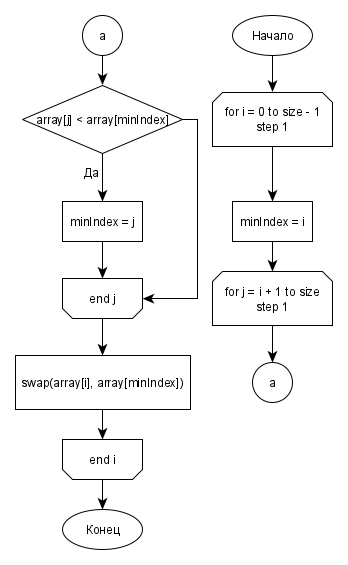
\includegraphics[width=0.7\linewidth]{../Рисунки/selection}
	\caption{Схема сортировки выбором}
	\label{fig:selection}
\end{figure}